\section{Простые вычисления (Задание 2 вариант 7)}

\subsection{Условие задания}

Вычислить: $\frac{y^2 sin (x^2)}{x + y^2}$

Приложение должно содержать следующие компоненты:

\begin{enumerate}
    \item{Заголовок формы должен отражать суть задания.}
    \item{Все элементы формы должны быть внятно подписаны (кнопки подписаны, у тестового поля должно быть написано, для чего оно нужно и т. д.)}
    \item{В коде должны быть комментарии и отступы (код должен быть легко читаем).}
    \item{Должна быть проверка ошибок --- ввод не числа, ввод числа, находящегося за пределами ОДЗ, ввод числа, принадлежащего ОДЗ.}
    \item{Если надо ввести 2 значения, то в случае ввод букв в оба поля, ошибка должна быть у обоих полей; в случае ввода одной буквы --- только у того поля, где буква.}
\end{enumerate}

\subsection{Вид формы в конструкторе}

Форма имеет вид (рис.\ref{fig:FormInConstruct2}):

\begin{figure}[!h]
    \centering
    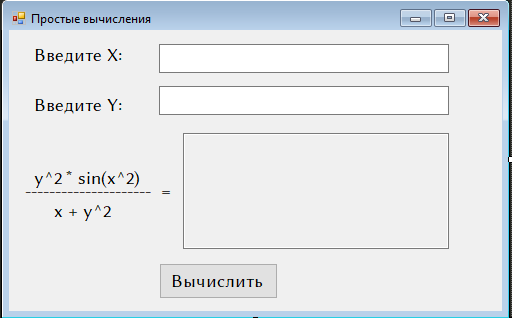
\includegraphics[width = 0.7\textwidth]{images/Task2/FormInConstructor.png}
    \caption{Вид формы в конструкторе}
    \label{fig:FormInConstruct2}
\end{figure}

\subsection{Таблица с описанием переименовнных элементов формы}

Все элементы формы были переименованы и их атрибыты изменены. Проведенные изменения представлены в таблице \ref{tab:label2}

\begin{longtable}[!h]{|l|l|l|}
    \caption{Значения атрибутов элементов в приложении <<Простые вычисления>>}
    \label{tab:label2}
    \hline
    \makecell{$\textbf{Описание элементов}$\\ $\textbf{формы}$}& \makecell{$\textbf{Список измененных}$\\ $\textbf{атрибутов}$}& \makecell{$\textbf{Новое значение}$\\ $\textbf{атрибута}$}\\ 
    \hline
    \makecell{Форма}& \makecell{Text}& \makecell{Простые вычисления}\\ 
    \hline
    \makecell{Первая надпись (label)}& \makecell{Name}& \makecell{lblInputX}\\ 
    \hline
    \makecell{Первая надпись (label)}& \makecell{Text}& \makecell{Введите X:}\\ 
    \hline
    \makecell{Вторая надпись (label)}& \makecell{Name}& \makecell{lblInputY}\\ 
    \hline
    \makecell{Вторая надпись (label)}& \makecell{Text}& \makecell{Введите Y:}\\ 
    \hline
    \makecell{Третья надпись (label)}& \makecell{Name}& \makecell{lblFormula1}\\ 
    \hline
    \makecell{Третья надпись (label)}& \makecell{Text}& \makecell{$x^2 * sin(x^2)$}\\ 
    \hline
    \makecell{Четвёртая надпись (label)}& \makecell{Name}& \makecell{lblFormula2}\\ 
    \hline
    \makecell{Четвёртая надпись (label)}& \makecell{Text}& \makecell{$-------$\\$-------$\\$-------  =$}\\ 
    \hline
    \makecell{Пятая надпись (label)}& \makecell{Name}& \makecell{lblFormula3}\\ 
    \hline
    \makecell{Пятая надпись (label)}& \makecell{Text}& \makecell{$x + y^2$}\\ 
    \hline

    \makecell{Первое текстовое поле (textBox)}& \makecell{Name}& \makecell{txtInX}\\ 
    \hline
    \makecell{Второе текстовое поле (textBox)}& \makecell{Name}& \makecell{txtInY}\\ 
    \hline
    \makecell{Третье текстовое поле (textBox)}& \makecell{Name}& \makecell{txtOut}\\ 
    \hline
    \makecell{Третье текстовое поле (textBox)}& \makecell{ReadOnly}& \makecell{True}\\ 
    \hline
    \makecell{Кнопка (button)}& \makecell{Name}& \makecell{btnStart}\\ 
    \hline
    \makecell{Кнопка (button)}& \makecell{Text}& \makecell{Вычислить}\\ 
    \hline
    \makecell{Обработчик ошибок 1\\ (errorProvider)}& \makecell{Name}& \makecell{errPrX}\\ 
    \hline
    \makecell{Обработчик ошибок 2\\ (errorProvider)}& \makecell{Name}& \makecell{errPrY}\\ 
    \hline
\end{longtable}

\subsection{Примеры работы}

При запуске приложения на экране появляется окно (рис.\ref{fig:StartForm2}).

\begin{figure}[!h]
    \centering
    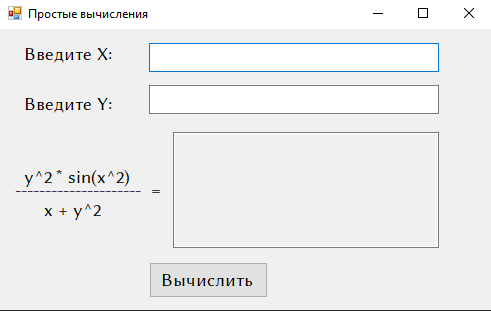
\includegraphics[width = 0.6\textwidth]{images/Task2/Start.png}
    \caption{Запуск приложения}
    \label{fig:StartForm2}
\end{figure}

\vspace{3cm}
При запуске с корректными данными (рис.\ref{fig:WorkForm2})

\begin{figure}[!h]
    \centering
    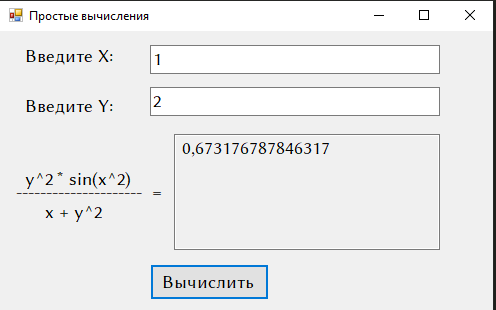
\includegraphics[width = 0.6\textwidth]{images/Task2/Works1.png}
    \caption{Запуск с корректными данными}
    \label{fig:WorkForm2}
\end{figure}

При запуске с некорректными данными (рис.\ref{fig:BadInputNotIntForm2})

\begin{figure}[!h]
    \centering
    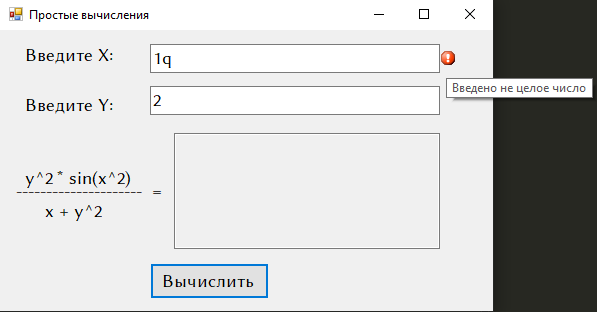
\includegraphics[width = 0.6\textwidth]{images/Task2/BadInputNotInt1.png}
    \caption{Запуск с некорректными данными}
    \label{fig:BadInputNotIntForm2}
\end{figure}

\subsection{Примеры кода}

Функция подсчета формулы с введенными значениями переменных:

\begin{minted}{c++}
double solve(long long x, long long y) {
	return (y * y * sin(x * x) * 1.0) / (x + y*y) ;
}
\end{minted}

Функция очистки полей:

\begin{minted}{c++}
	private: void ClearAll() { // очистка полей
		this->txtOut->Text = "";
		errPrX->SetError(txtInX, String::Empty);
		errPrY->SetError(txtInY, String::Empty);
	}
\end{minted}

Другие фрагменты кода расположены в приложении \ref{app:task2}. Полный код программы приведен в приложении \ref{app:zip}
